\documentclass[]{report}
\usepackage{graphicx}
\usepackage[left=0.75in,top=0.55in,right=0.75in,bottom=0.7in]{geometry}

% Title Page
\title{CS 251 Lab 09}
\author{Group 02\\ Harshal Mahajan, Tanmay Parekh, Navneet Agarwal}
\date{October 3, 2015}

\begin{document}
\maketitle

\begin{abstract}
\section*{Profiling Graphs}
The following outputs were generated on optimizations applied during the debug mode of the Box2d.
\\ \\
\subsection{Debug Mode}
\subsection*{No Change in the code}
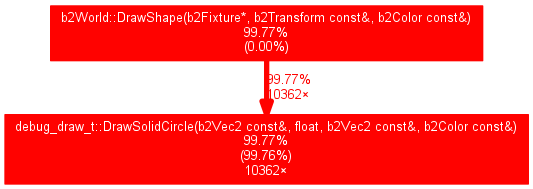
\includegraphics[width=1\textwidth]{callgraph1.png}
As the above call graph clearly shows, the majority of the time is consumed in DrawSolidCircle function during execution. On further inspection we can see that in the function DrawSolidCircle there is a for loop which has no function to perform.
On commenting that te code becomes much faster. The following call graph was generated later.
\\ \\
\subsection*{Code Changed}
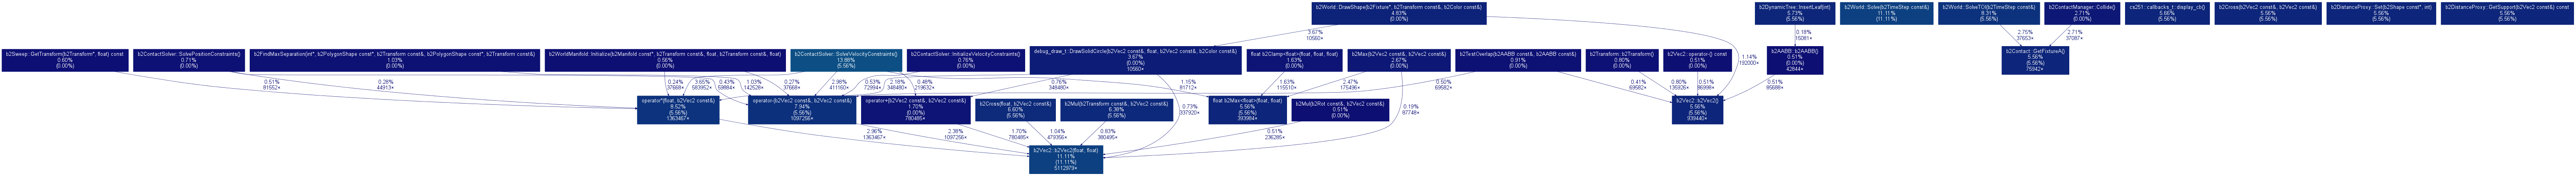
\includegraphics[width=1\textwidth]{callgraph.png}
The change imbibed in the code is the for loop in DrawSolidcircle in render.cpp which was iterated without function for 300000 times. The graph is clearly not visible as the rest functions have time comparable to the DrawShape and the rest functions. However the first 5 functions in this case are
\begin{itemize}
\item $b2Vec2::b2Vec2(float, float)$
\item $b2World::Solve(b2TimeStep const\&)$
\item $operator*(float, b2Vec2 const\&)$
\item $operator-(b2Vec2 const\&, b2Vec2 const\&)$
\item $float b2Max<float>(float, float)$
\item $b2Contact::GetFixtureA()$
\end{itemize}
\newpage
\subsection{Release Mode}
\subsection*{No Change in the code \& No Optimizations}
Under no optimizations the code takes time longer than that in the debug mode for the identical conditions.
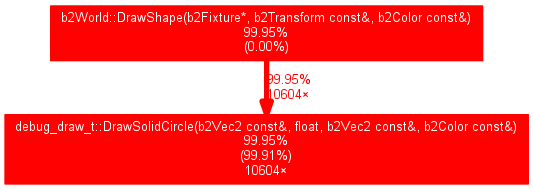
\includegraphics[width=1\textwidth]{callgraph2.png}
\\ \\
\subsection*{Code Changed \& No optimization}
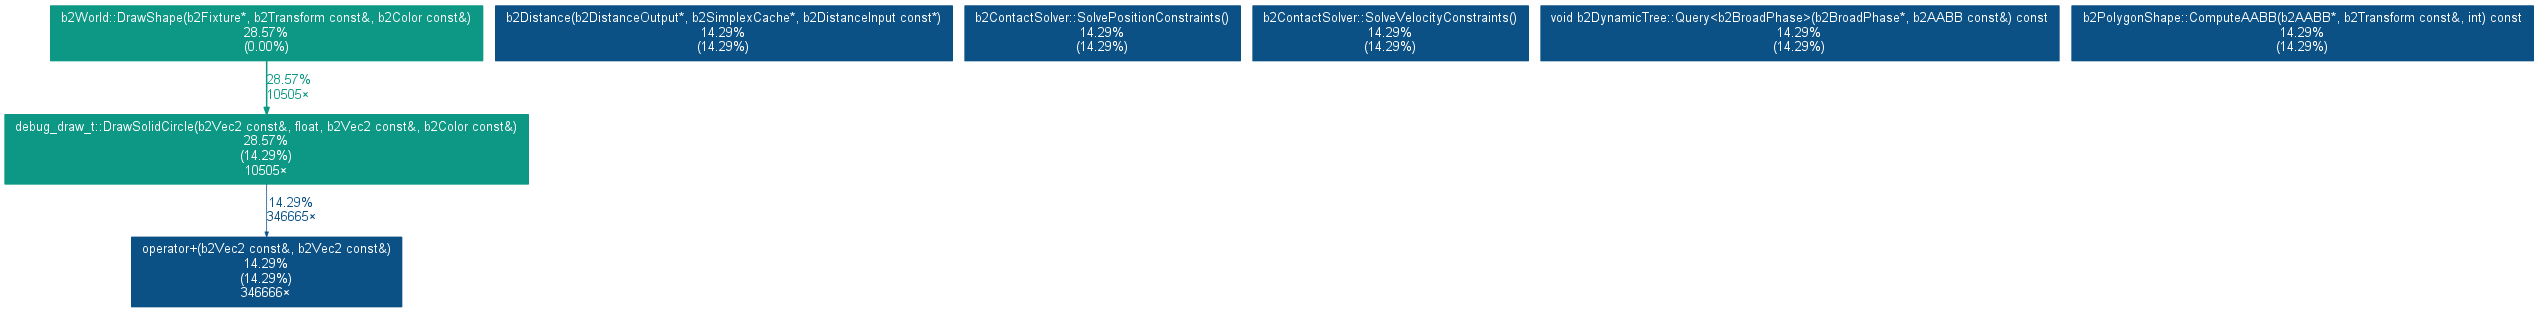
\includegraphics[width=1\textwidth]{callgraph3.png}
The call graph is again not clearly visible and there is no way to display these graphs clearly on one page. However the most time consuming functions in this part are the the following functions each taking negligible time compared to no changes in the code.
\begin{itemize}
\item $operator+(b2Vec2 const\&, b2Vec2 const\&)$
\item $debug\_draw\_t::DrawSolidCircle(b2Vec2 const\&, float, b2Vec2 const\&, b2Color const\&)$
\item $b2Distance(b2DistanceOutput*, b2SimplexCache*, b2DistanceInput const*)$ 
\item $b2ContactSolver::SolvePositionConstraints()$
\item $b2ContactSolver::SolveVelocityConstraints()$
\item $void b2DynamicTree::Query<b2BroadPhase>(b2BroadPhase*, b2AABB const\&) const$
\item $b2PolygonShape::ComputeAABB(b2AABB*, b2Transform const\&, int) const$
\\ \\
\end{itemize}
\newpage
\subsection*{No Change in the code with Optimizations}
The code is well branched under optimizations abd the call stack is completely used. The functions called are:
\\ \\
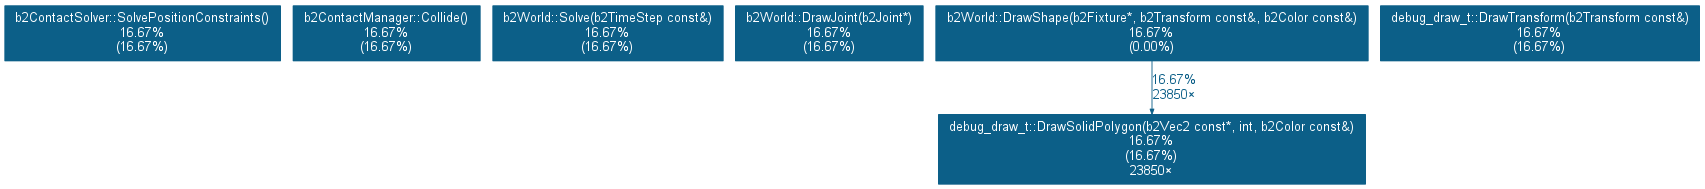
\includegraphics[width=1\textwidth]{callgraph4.png}
\begin{itemize}
\item $b2ContactSolver::SolvePositionConstraints()$
\item $b2ContactManager::Collide()$
\item $b2World::Solve(b2TimeStep const\&)$
\item $b2World::DrawJoint(b2Joint*)$
\item $debug\_draw\_t::DrawSolidPolygon(b2Vec2 const*, int, b2Color const\&)$
\end{itemize}

\subsection*{Code changed with Optimizations}
The code is well branched under optimizations abd the call stack is completely used, time taken is minimal. The functions called are:
\\ \\
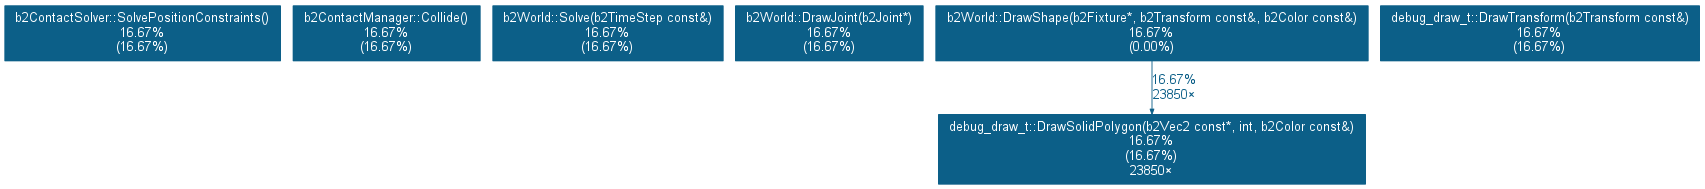
\includegraphics[width=1\textwidth]{callgraph4.png}
\begin{itemize}
\item $debug\_draw\_t::DrawSolidPolygon(b2Vec2 const*, int, b2Color const\&)$
\item $b2ContactSolver::SolveVelocityConstraints()$
\item $b2World::DrawDebugData()$
\item $b2World::Solve(b2TimeStep const\&)$
\item $debug\_draw\_t::DrawSegment(b2Vec2 const*, int, b2Color const\&)$
\end{itemize}
\section*{Interesting Observations}
\begin{itemize}
\item The Optimization increases the calls made by a function.
\item The call graph ignores all the function whose timing is nominals as compared to the rest
\end{itemize}
\end{abstract}

\end{document}          
